\chapter{Flow Matching \& SD3}

Un modello generativo ha lo scopo di modellare la distribuzione di probabilità di un insieme di dati. Se abbiamo un dataset con i seguenti dati osservati $\{x^{(1)},x^{(2)},\,\dots\,,x^{(N)}\}$, l'obbiettivo sarà quello di imparare una distribuzione in modo tale che:
\[
    p_{\operatorname{model}}(x)\approx p_{\operatorname{data}}(x)
\]

Dove $p_{\operatorname{data}}(x)$ è la distribuzione reale da cui i dati sono stati campionati, a noi sconosciuta, mentre $p_{\operatorname{model}}(x)$ è la distribuzione appresa dal modello generativo. Una volta appresa possiamo ottenere nuovi dati realistici, simili a quelli presenti nel dataset, stimare quanto è plausibile un nuovo dato, completare dati come riempire le parti mancanti in un'immagine o in una frase e condizionare la generazione su un'informazione generando per esempio una didascalia a partire da un'immagine.

\section{Mappatura diretta e Processi di Markov}
Un primo approccio consiste in una \textbf{mappatura diretta} tramite un modello deterministico $f: \mathbb{R}^d \to \mathbb{R}^d$ tale che $x_1 = f(x_0)$, dove $x_0 \sim p_{\operatorname{data}}(x)$. Questo approccio funziona, ma è rigido: per fenomeni complessi (come immagini ad alta dimensione), non basta una mappa unica, serve un processo graduale e continuo, che trasformi progressivamente una distribuzione in un’altra. È qui che entra in gioco il concetto di flusso continuo, modellato come un processo di Markov continuo nel tempo, dove lo stato evolve secondo una certa velocità $v_t(x)$

\section{Flusso e Velocità}
Il \textbf{flusso} è il modo in cui la distribuzione cambia nel tempo. Ogni punto $x$ "si muove" nello spazio dei dati seguendo un campo di velocità $v_t(x)$. La dinamica è modellata tramite un'equazione differenziale ordinaria (ODE):
\begin{equation}
    \frac{dx}{dt} = v_t(x), \quad x(0) \sim p_{\operatorname{data}}(x)
\end{equation}

Quindi il modello impara come spostare i punti nel tempo per trasformare una distribuzione iniziale $p_0$ (es. rumore gaussiano) in una distribuzione finale $p_1$ (es. immagini reali).

\section{I modelli da cui ci discostiamo}

Affrontiamo in breve i modelli da cui ci discostiamo per poter giungere all'idea del \textbf{Flow Matching} con una base più solida. In primis ci sono i modelli di Stable Diffusion, già approfonditi nel capitolo~\label{chapter15}, essi si basano sulla costruzione e ricostruzione di un'immagine su flussi stocastici. Questi flussi sono diversi da quelli citati tramite le equazioni differenziali ordinarie, poiché segueno un approccio probabilistico invece di un approccio deterministico. Oltre a questi ci sono i \textit{Normalizing Flows} e i \textit{Continuous Normalizing Flows}

\subsection{Normalizing Flows}
I \textbf{Normalizing Flows} (NF) invece sono deterministici e invertibili. Essi trasformano una distribuzione semplice (e.g una gaussiana) in una complessa (e.g immagini) usando trasformazioni invertibili $f_\theta$. Si può quindi calcolare esattamente la densità risultante grazie al cambiamento di variabili:

\begin{equation}
    \log p(x) = \log p_z(f_\theta^{-1}(x)) + \log \left|\det\left(\frac{\partial f_\theta^{-1}(x)}{\partial x}\right)\right|
\end{equation}
Il limite di questi modelli è la complessità del calcolo del determinante jacobiano, che rende difficile scalare a reti profonde.

\subsection{Continuous Normalizing Flows}
Per superare il limite del determinante, i Continuous Normalizing Flows (CNF)~\cite{} modellano la trasformazione come un flusso continuo nel tempo:

\begin{equation}
    \frac{dx}{dt} =f_\theta(x,t)
\end{equation}

In pratica, usano un’ODE per "spingere" la distribuzione nel tempo. Il vantaggio è che il log-determinante del Jacobiano può essere calcolato in modo più efficiente come integrale nel tempo (usando l’equazione di continuità).
%Fonte: Chen et al., "Neural Ordinary Differential Equations", NeurIPS 2018

\section{Flow Matching}
Il \textbf{Flow Matching} (FM)~\cite{lipman2023flow} nasce come una via di mezzo tra i modelli di diffusione (stocastici) e i CNF (deterministici). Invece di simulare flussi completi e calcolare likelihood complesse, il Flow Matching: impara direttamente il campo di velocità $v_t(x)$ che collega le due distribuzioni. Immaginiamo di voler insegnare a un'auto a guida autonoma ad andare dal punto $x_0$ (rumore) al punto $x_1$ (immagine di un gatto), il modello traccerà una linea retta da $x_0$ a $x_1$. Poi posizionerà l'auto in un punto qualsiasi di questa linea $\gamma_t$ e le viene chiesto quale sia la direzione e la velocità esatta per rimanere su questa linea (velocità target $v_t$), che il modello proverà a indovinare($\hat{v}_t$.

\subsection{Loss di Flow Matching}
La \textbf{Flow Matching Loss} diventa molto intuitiva a seguito di questa osservazione:
\begin{equation}
    \mathcal{L}_{FM} = \mathbb{E}_{x_0,x_1,t} \left[ \left\| \hat{v}_t(\gamma_t) - v_t(\gamma_t) \right\|^2 \right]
\end{equation}

La $\hat{v}_t(\gamma_t)$ è la velocità predetta dal modello, mentre la $v_t(\gamma_t)$ è la velocità corretta, che conosciamo bene poiché abbiamo definito noi il percorso rettilineo. La loss misura semplicemente la differenza tra la previsione del modello e la realtà. L'obiettivo è minimizzare questo errore, cioè insegnare al modello a dare sempre le istruzioni di guida corrette per seguire il percorso semplice che gli abbiamo imposto. Addestrare il modello su punti intermedi ($\gamma_t$) lungo il percorso, e non solo agli estremi, rende l'apprendimento molto più stabile ed efficiente. È come fare delle correzioni a un guidatore a metà curva, invece di aspettare che arrivi a destinazione per dirgli che ha sbagliato tutto.

\subsection{Marginalization Trick}

L’obiettivo del Marginalization Trick è evitare di campionare intere traiettorie e calcolare le velocità target in modo efficiente. Invece di definire una loss sulla traiettoria completa tra $x_0$ e $x_1$, si considera la distribuzione condizionata $\psi_t(x | x_0, x_1)$, che definisce la probabilità di essere in un certo punto $\gamma_t$ lungo il percorso e calcoliamo esattamente quale dovrebbe essere la sua velocità in quel punto per rimanere sulla rotta, una volta fatto ciò marginelizzerò il processo. Questo approccio consente un calcolo efficiente dei target di velocità senza dover simulare interamente le traiettorie, ma farmi un'idea in base ai punti casuali campionati.

\begin{equation}
    \mathcal{L}_{FM} =\mathbb{E}_{x_0,x_1}\left[\mathbb{E}_t\left[\mathbb{E}_{\gamma_t\sim\psi_t(\cdot|x_0,x_1)}\|f_\theta(\gamma_t,t) - v_t(\gamma_t|x_0,x_1)\|^2\right]\right]
\end{equation}
L'addestramento diventa un compito molto più semplice e veloce. Non dobbiamo risolvere equazioni differenziali complesse durante il training, ma solo fare un semplice calcolo puntuale.

\subsection{Percorsi Affini e Gaussiani}
Il parametro $\gamma_t$ può essere calcolato anche tramite degli studi differenti, tramite l'utilizzo dei Percorsi Affini o quelli Gaussiani:

\subsubsection{Percorso affine}
Sono le traiettorie lineari definite come:
\begin{equation}
    \gamma_t = (1-t)\,x_0 + t\,x_1
\end{equation}
Questa è la via più semplice immaginabile: una linea retta a velocità costante. È come tracciare una linea con un righello tra il punto di partenza e quello di arrivo. È prevedibile, facile da calcolare e perfetto per insegnare al modello la direzione generale del movimento. La velocità in ogni punto di questo percorso è semplicemente $x_1-x_0$.

\subsubsection{Percorso Gaussiano}

\begin{equation}
    \gamma_t = (1-t)\,x_0 + t\,x_1 + \sqrt{t\,(1-t)}\cdot\epsilon, \qquad \epsilon\sim\mathcal{N}(0,I)
\end{equation}
Questo percorso è una linea retta a cui viene aggiunto un po' di rumore casuale (gaussiano). La quantità di rumore è massima a metà percorso ($t=0.5$) e zero agli estremi. È come se fosse un aereo che vola da una città all'altra. La rotta principale è una linea retta, ma piccole turbolenze lo fanno deviare leggermente. Questo rende il modello più robusto. Impara non solo a correggere la rotta quando si trova esattamente sulla linea retta, ma anche quando è un po' fuori rotta. Questo lo prepara meglio a gestire situazioni complesse durante la generazione vera e propria, rendendolo più simile ai modelli a diffusione.

\subsection{Metodologia di Addestramento}
Ci sono ben tre tipologie di addestramento per il Flow Matching, le quali sono descritte in breve quì di seguito:
\begin{itemize}
    \item \textbf{Simulation-Free:} il flusso è definito direttamente tramite la specifica del percorso di probabilità e ottimizzando il campo vettoriale di conseguenza, evitando delle simulazioni costose;
    \item \textbf{Gradient-Based:} ottimizzazione con discesa del gradiente per ottimizzare i parametri;
    \item \textbf{Conditional Flow Matching:} il flow matching definisce una funzione obbiettivo chiamata; \textbf{Conditional Flow Matching Objective}, la quale garantisce stime prive di bias dei gradienti e un efficiente allenamento.
\end{itemize}

Come abbiamo potuto vedere solitamente ci troviamo in una situazione in cui abbiamo due distribuzioni: una inziale e una target. Ovviamente per giungere da una all'altra ci saranno delle fasi intermedie, e vi è una procedura di training che viene adottata. Inizialmente si prendono in considerazione in maniera casuale coppie di punti rispettivamente uno della distribuzione inziale e uno della distribuzione target, e muoviamo questi punti lungo una traiettoria rettilinea a una velocità costante, pratica visualizzabile in Figura~\ref{fig:FMTrain}.
\begin{figure}
    \centering
    \includegraphics[width=0.5\textwidth]{figure/FMTrain.png}
    \caption{Visualizzazione 3D della procedura di Training, in blu la distribuzione iniziale dei datapoint, in arancione la distribuzione target.}
    \label{fig:FMTrain}
\end{figure}
Il Problema della Confusione è una difficoltà, nel momento in cui accoppiamo due punti fra rumore e target, i loro percorsi rettilinei quasi certamente si incroceranno. Nel punto di incrocio, il modello riceve segnali contraddittori non sapendo quale traiettoria seguire. Però il modello non è progettato per imparare i percorsi individuali dei singoli punti. È progettato per imparare il campo di velocità complessivo, cioè la "mappa del vento" che sposta l'intera distribuzione (la nuvola di punti) da una forma all'altra. È un po' come versiamo una caraffa d'acqua (distribuzione iniziale) in un bicchiere (distribuzione target). Se seguissimo due gocce d'acqua a caso, i loro percorsi saranno caotici e si incroceranno. Ma il flusso complessivo dell'acqua ha una direzione chiara e non si "incrocia" con se stesso. Il modello neurale, vedendo milioni di esempi di gocce, ignora il caos individuale e impara il flusso aggregato e liscio del liquido. Il codice di seguito nella classe \texttt{VelocityNet} è il "cervello" che impara questa mappa del vento. Prende in input una posizione x e un tempo t e restituisce la velocità che un punto dovrebbe avere in quel punto dello spazio-tempo

\begin{python}[frame=trBL]
import torch.nn as nn
import torch.nn.functional as F

class VelocityNet(nn.Module):
    def __init__(self, input_dim, h_dim=64):
        super().__init__()
        self.fc_in  = nn.Linear(input_dim + 1, h_dim)
        self.fc2    = nn.Linear(h_dim, h_dim)
        self.fc3    = nn.Linear(h_dim, h_dim)
        self.fc_out = nn.Linear(h_dim, input_dim)
    
    def forward(self, x, t, act=F.gelu):
        t = t.expand(x.size(0), 1)  
        # Ensure t has the correct dimensions
        x = torch.cat([x, t], dim=1)
        x = act(self.fc_in(x))
        x = act(self.fc2(x))
        x = act(self.fc3(x))
        return self.fc_out(x)

# Instantiate the model
input_dim = 2
model = VelocityNet(input_dim)
\end{python}

La parte più complessa del Flow Matching è la maniera attraverso la quale alleniamo questa rete, per ogni training step dobbiamo seguire i seguenti step:

\begin{enumerate}
    \item Campionare punti casuali dalle distribuzioni di origine e di destinazione e accoppiare i punti;
    \item Campionare tempi casuali compresi tra 0 e 1;
    \item  Calcolare le posizioni in cui questi punti si troverebbero in quei momenti se si muovessero a velocità costante dalla sorgente al bersaglio;
    \item Calcolare la velocità che avrebbero in quei punti se si muovessero a velocità costante, questa cosa viene effettuata dalla rete neurale, per tanto dovrà scoprire da se la velocità costante;
    \item Addestrare la rete a prevedere queste velocità, che finiranno per "cercare la media" quando la rete dovrà fare lo stesso per molti, molti punti.
\end{enumerate}

\begin{figure}[hbtp]
    \centering
    \includegraphics[width=0.8\textwidth]{figure/TrajFM}
    \caption{Rappresentazione di ciò che accade dopo il training alle traiettorie che seguiranno i punti fino a giungere alla distribuzione target.}
    \label{fig:trajFM}
\end{figure}

Anche se le traiettorie risultino essere lisce e non incrociate, la loro curvatura significa che dobbiamo integrare lentamente e con attenzione per evitare di accumulare errori significativi. Ci sono stati dei paper i quali hanno approfondito questo dettaglio~\cite{lipman2023flow}, offrendo un modo efficace per accelerare l'integrazione "raddrizzando" le traiettorie curve, attraverso un metodo che chiamano \textbf{Reflow}.

\subsection{Reflow}

Una volta addestrato, il nostro modello ha imparato un campo di velocità che produce traiettorie lisce ma spesso curve. Per seguire una curva con precisione, bisogna fare tanti piccoli passi, rendendo la generazione (inferenza) molto lenta. Il \textbf{Reflow} è il processo che si occupa di migliorare questo flusso permettendo di "raddrizzare" queste curve.

\begin{enumerate}
    \item \textbf{Primo Giro:} Addestriamo il modello con percorsi rettilinei e otteniamo un modello che genera traiettorie curve ma corrette (come prima;
    \item \textbf{Secondo Giro:} Applico il Reflow, usiamo il modello del primo giro per generare una traiettoria completa da un punto $x_0$ a un punto finale simulato $x_1'$. Questa traiettoria sarà curva;
    \item \textbf{Nuovo addestramento:} Dimentichiamo il percorso curvo e addestriamo un nuovo modello (o riaddestriamo lo stesso) dicendogli: di imparare la linea retta tra $x_0$ e questo nuovo punto finale $x_1'$.
\end{enumerate}

Facendo in questo modo, il modello imparerà percorsi che sono intrinsecamente più dritti. Percorsi più dritti significano che possiamo usare meno passi per integrarli, rendendo la generazione molto più veloce (Figura~\ref{fig:reflow}).
\begin{figure}
    \centering
    \includegraphics[width=0.7\textwidth]{figure/Reflow}
    \caption{Idea alla base del Reflow, per la considerazione del raggiungimento ai punti target.}
    \label{fig:reflow}
\end{figure}
Ci sono numerose animazioni le quali mettono in luce come sia diretto, ma soprattuto le traiettorie con l'utilizzo del Reflow, siano molto più lineari rispetto a quelle prive di esso, inoltre il passaggio dalle configurazioni iniziali a quelle finali nel Flow Matching, subiscono una sorta di aggregamento iniziale prima di giungere nella posizione finale, cosa che non succede con il Reflow, le quali vanno direttamente nella posizione finale dei valori target.

\subsection{Condizionamento nei Modelli Generativi}

In scenari controllati, si desidera che il modello generi output coerenti con un certo input. Questo si ottiene introducendo dei \textbf{Condizionamenti} nella funzione di costo o nella dinamica del modello, utilizzando la \textbf{Guidance}. Un meccanismo che modifica il processo di generazione per ottenere campioni che appartengano a una distribuzione condizionata $p(x|y)$, anche quando il modello è stato addestrato sulla distribuzione marginale $p(x)$ non condizionata. Supponiamo di avere un generatore molto bravo a generare immagini relaistiche di cani, modellando bene $p(x)$, ma vogliamo generare solo Husky identificati come $y$ (Figura~\ref{fig:Guidance}), in questi casi la \textbf{Guidance} ci permette di "spingere" la generazione verso i campioni che hanno un'alta probabilità condizionata da noi desiderata, senza dover riaddestrare la rete da zero, ci sono due tipologie principali di Guidance, la \textit{Classifier Guidance} e la \textit{Classifier-Free Guidance}.

\begin{figure}
    \centering
    \includegraphics[width=0.6\textwidth]{figure/Guidance}
    \caption{Rappresentazione della Guidance, avendo un modello il quale ci restituisce immagini realistiche di cani, ma vogliamo forzare che ci dia come esito foto di Husky.}
    \label{fig:Guidance}
\end{figure}

\subsubsection{Classifier Guidance}

Durante la generazione, a ogni passo, chiediamo a un classificatore di immagini già addestrato $p_\eta(y\,|\,x)$ (un modello separato addestrato a riconoscere le razze di cani) di guardare l'immagine parzialmente formata. Il classificatore non fa altro che dire in quale direzione modificare i pixel per ottenere il risultato desiderato. Il campo di velocità del nostro modello viene quindi "spinto" un po' in quella direzione.

\begin{equation}
    \nabla_x\log p(x\,|\,y) = \nabla_x\log p(x) + \nabla_x \log p_\eta (y\,|\,x)
\end{equation}
Richiedere un classificatore esterno, potrebbe portare a non essere perfetto o non allineato con il modello generativo, e non sarebbe un bene nella procedura di training complessiva.

\subsubsection{Classifier-Free Guidance}

Durante l'addestramento, insegniamo al modello due cose contemporaneamente, la prima si basa sul come generare un'immagine senza alcuna condizione, la seconda come generare un'immagine con un condizionamento. Durante la generazione, fondiamo le due modalità e calcoliamo la direzione effettuando una media pesata. Il parametro $w$ controlla l'intensità della guida: un $w$ alto significa basarsi esclusivamente sul condizionamento.

\begin{equation}
    \nabla_x\log \hat{p}(x\,|\,y) = (1 - w)\nabla_x\log p(x) + w\,\nabla_x \log p (y\,|\,x)
\end{equation}

Il vantaggio che si ha è una stabilità e un'efficacia maggiore perché l'abilità di essere guidato è integrata direttamente nel modello. Non c'è bisogno di un "esperto" esterno.

\subsubsection{Guidance nel Flow Matching}
Nel Flow Matching invece dei gradienti log-probabilistici detti anche score, si lavora con campi di velocità $u_t(x)$ avendo variazioni sia per quella con classificatore che per quella senza classificatore come visibile di seguito:
\begin{equation*}
    \hat{u}_t(x\,|\,y) = u_t(x) + w\,b_t\nabla_x \log p_\eta(y\,|\,x)
\end{equation*}
\begin{equation*}
    \hat{u}_t(x\,|\,y) =(1-w)\,u_t(x) + w\,u_t(x\,|\,y)
\end{equation*}

\section{T5}

\textbf{T5} sta per \textbf{Text-To-Text Transfer Transformer}, ed è un modello sviluppato da Google Research nel 2020~\cite{raffel2020t5}, il suo concetto chiave è molto semplice, ma potente, ossia quello che tutti i compiti di \textit{Natural Language Processing}, sono formulati come trasformazioni di testo in testo.

\begin{table}[htbp]
\centering
\begin{adjustbox}{width=0.9\textwidth}
\begin{tabular}{|l|p{7cm}|l|}
\hline
\textbf{Task} & \textbf{Input} & \textbf{Output} \\
\hline
Traduzione & \texttt{translate English to German: How are you?} & \texttt{Wie geht es dir?} \\
\hline
Riassunto & \texttt{summarize: The book was about...} & \texttt{It was a book about...} \\
\hline
Classificazione & \texttt{classify sentiment: I love this movie!} & \texttt{positive} \\
\hline
Domanda-Risposta & \texttt{question: What is the capital of France? context: France is a country\dots} & \texttt{Paris} \\
\hline
\end{tabular}
\end{adjustbox}
\caption{Esempi di task gestiti da T5 con input testuali specifici, quì tutto è testo in input, e tutto è testo in output.}
\end{table}
T5 usa un'architettura Transformer Encoder-Decoder, simile a quella dei modelli di traduzione neurale~\cite{vaswani2017attention}, l'Encoder legge l'input testuale e lo rappresenta come sequenza di vettori, mentre il Decoder genera l'output testuale token per token, usando l'attenzione sui vettori prodotti dall'Encoder, dunque è diverso da BERT e GPT come abbiamo visto nel capitolo~\ref{cap:14} poiché è come se combini i due modelli.

\subsection{Masked Attention}
T5 utilizza la \textbf{Masked Attention}, nella self-attention classica ogni token può guardare tutti gli altri token della sequenza. In questo caso i token, non possono guardare in avanti nella sequenza, nel Decoder si genera un testo token per token e durante l'addestramento si ha già tutto l'output target a disposizione, ma bisogna impedire che il modello effettui delle scorrettezze guardando ai token futuri.

\subsection{Obbiettivi di Training}

T5 non è addestrato su una Next-Token Prediction o Masked Token Prediction Standard, invece è addestrato sulla \textbf{Span Corruption}, la quale rimuove casualmente degli span (frammenti di testo) dal testo, facendo diventare l'input il testo con span mascherati. L'output saranno gli span rimossi, permettendo al modello di imparare a ricostruire il testo, la forza di T5 è anche quella di essere allenato su uno dei dataset più puliti e grandi disponibili al momento, chiamato C4 Dataset (Colossal Clean Crawled Corpus), inoltre dopo il pre-training viene effettuato un fine-tuning su dei task specifici come la traduzione, il riassunto, ecc\dots

\section{DiT}
\textbf{DiT} è un \textbf{Vision Transformer}~\cite{dosovitskiy2021vit}, questi trattano un'immagine come una sequenza di patch (piccoli blocchi dell'immagine) e la elaborano come se fosse una frase, usando un Transformer (Figura~\ref{fig:ViT}). DiT tuttavia è addestrato sui documenti come immagini~\cite{li2023dit}, progettato per comprendere la struttura e il contenuto visivo di documenti senza testo esplicito.
\begin{figure}
    \centering
    \includegraphics[width=0.7\textwidth]{figure/VisionTransformer}
    \caption{Panoramica del modello. Dividiamo un'immagine in patch di dimensioni fisse, incorporiamo linearmente ciascuna di esse, aggiungiamo le incorporazioni di posizione e diamo la sequenza di vettori risultante a un codificatore Transformer. Eseguendo la classificazione, utilizziamo l'aggiunta di un "token di classificazione" apprendibile dalla sequenza.}
    \label{fig:ViT}
\end{figure}
DiT utilizza la stessa struttura dei Vision Transformer, l'immagine del documento viene divisa in patch, e ognuno di questi patch diventa un embedding, gli embedding vengono processati da stack di Transformer encoder, e come nel ViT, c'è un [CLS] token il cui embedding finale può essere usato per classificazione o altre task globali.

\section{MMDiT}

\textbf{MMDiT} è un'estensione di DiT che integra testi e immagini in un unico framework Transformer~\cite{zhang2023mmdetdit}, è pensato per task multimodali, come la comprensione congiunta del layout e del contenuto testuale.

\begin{table}[htbp]
\centering
\begin{adjustbox}{width=0.9\textwidth}
\begin{tabular}{|l|p{5.5cm}|p{6cm}|}
\hline
\textbf{Caratteristica} & \textbf{DiT} & \textbf{MMDiT} \\
\hline
Modalità input & Solo immagine & Immagine + Testo \\
\hline
Architettura base & Vision Transformer & Multimodal Transformer (visivo + testuale) \\
\hline
Positional embedding & 2D patches & 2D patches + 2D bounding box \\
\hline
Addestramento & Supervised / Self-supervised & Multimodal supervision \\
\hline
Vantaggi & No OCR necessario & Più preciso nei task semantici \\
\hline
Task principali & Layout, classificazione & VQA, estrazione, analisi semantica \\
\hline
\end{tabular}
\end{adjustbox}
\caption{Confronto tra DiT e MMDiT per la comprensione dei documenti.}
\end{table}

\section{SD3}

\textbf{SD3} invece è un modello di generazione condizionata di immagini basato sull'architettura dei modelli di diffusione~\cite{stablediffusion3}, rappresenta una delle più recenti evoluzioni di stable diffusion, ottimizzato per qualità, scalabilità e flessibilità d'uso in vari contesti multimodali, \textbf{SD3} (Stable Diffusion 3) è la terza generazione del modello \textit{Stable Diffusion}, rilasciata da Stability AI. È stato progettato per superare i limiti delle versioni precedenti, con un focus particolare sulla coerenza testuale, l'alta risoluzione, multi-condizionalità e la scalabilità. A differenza dei precedenti modelli, SD3 non è un puro modello di diffusione tradizionale, ma è influenzato dal paradigma \textbf{Flow Matching} affrontato in questo capitolo, questo significa che è in grado di impara una mappa deterministica dello spazio latente e l'immagine target, ispirandosi alla teoria del flusso. Utilizza T5 come modello di testo, avendo una vera e propria archiettutra a blocchi.
\vspace{0.8cm}
\begin{figure}[htbp]
    \centering
    \resizebox{0.8\textwidth}{!}{
    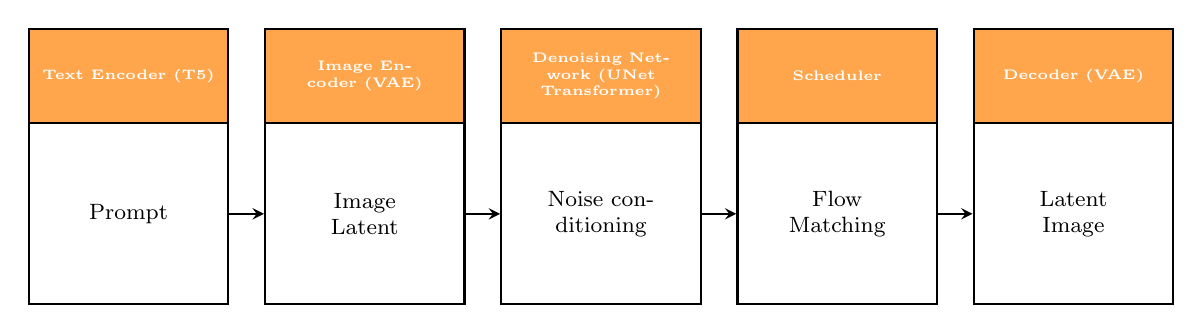
\begin{tikzpicture}[
    % Definizione degli stili
    main_block/.style={
        rectangle,
        draw=black,
        thick,
        minimum width=2.5cm,
        minimum height=3.5cm,
        fill=white
    },
    header/.style={
        rectangle,
        draw=black,
        thick,
        minimum width=2.5cm,
        minimum height=1.2cm,
        fill=orange!70,
        text=white,
        font=\tiny\bfseries,
        align=center,
        text width=2.3cm
    },
    content/.style={
        rectangle,
        draw=black,
        thick,
        minimum width=2.5cm,
        minimum height=2.3cm,
        fill=white,
        font=\footnotesize,
        align=center,
        text width=2.3cm
    },
    arrow/.style={
        ->,
        thick,
        >=stealth
    }
]

% Posizioni dei blocchi
\coordinate (pos1) at (0, 0);
\coordinate (pos2) at (3, 0);
\coordinate (pos3) at (6, 0);
\coordinate (pos4) at (9, 0);
\coordinate (pos5) at (12, 0);

% Blocco 1: Text Encoder
\node[header] (h1) at (pos1) {Text Encoder (T5)};
\node[content] (c1) at ([yshift=-1.75cm]pos1) {Prompt};

% Blocco 2: Image Encoder
\node[header] (h2) at (pos2) {Image Encoder (VAE)};
\node[content] (c2) at ([yshift=-1.75cm]pos2) {Image\\Latent};

% Blocco 3: Denoising Network
\node[header] (h3) at (pos3) {Denoising Network (UNet Transformer)};
\node[content] (c3) at ([yshift=-1.75cm]pos3) {Noise conditioning};

% Blocco 4: Scheduler
\node[header] (h4) at (pos4) {Scheduler};
\node[content] (c4) at ([yshift=-1.75cm]pos4) {Flow\\Matching};

% Blocco 5: Decoder
\node[header] (h5) at (pos5) {Decoder (VAE)};
\node[content] (c5) at ([yshift=-1.75cm]pos5) {Latent\\Image};

% Frecce tra i blocchi (verso destra)
\draw[arrow] (c1.east) -- (c2.west);
\draw[arrow] (c2.east) -- (c3.west);
\draw[arrow] (c3.east) -- (c4.west);
\draw[arrow] (c4.east) -- (c5.west);

\end{tikzpicture}}
    \caption{Schema della pipeline del modello di Stable Diffusion 3.}
\end{figure}

